\chapter{Predictive Coding}

\section{Introduction}

Predictive coding, in its current form, was formalized by \cite{rao1999predictive}. This theoretical neuroscience model posited that sensory processing is a filtering problem, in which latent states underlying the environmental stimuli are estimated according to their agreement with the observed input as well as prior beliefs about these quantities. This offered an explanation for ``extra-classical" receptive field effects in visual processing, in which stimuli outside the receptive field of a particular cortical neuron are able to affect that neuron's activity. This was explained as the result top-down prior beliefs.

However, the notion of perception as a generative process dates back to at least \cite{von1867handbuch}. \textit{TODO: mention other early work before Rao and Ballard with similar ideas}

Predictive coding claims that sensory processing, i.e. perception, is fundamentally about constructing a generative model of the input sensory signal. To perform \textit{inference} in this model (to perceive), the model uses its current estimate of the latent variables underlying the environment to generate reconstructions or predictions of the input. Using the residual (error) from this reconstruction or prediction, along with residuals from prior beliefs, the model updates its estimate of these latent variables. \textit{Learning} corresponds to updating the parameters of the generative model to improve these overall residuals.
\newline

\subsection{Literature Summary}

\noindent \cite{clark2013whatever} provides a survey of the area of predictive coding
\newline

\noindent \cite{friston2002functional, friston2003learning, friston2005theory} presents a free energy formulation of predictive coding that uses expectation maximization. Primarily focuses on the static setting. Puts forth a theory of cortical processing as carrying out predictive coding.
\newline

\noindent \cite{friston2003dynamic} presents \textit{dynamic causal modeling}.
\newline

\noindent \cite{friston2008variational} presents \textit{variational filtering}.
\newline

\noindent \cite{friston2008DEM} presents \textit{dynamic expectation maximization} (DEM).
\newline

\noindent \cite{friston2010generalised} presents \textit{generalized filtering}, which does not make the mean-field assumption and instead treats all unknown variables as conditionally dependent. This differs from variational filtering \cite{friston2008variational} in that it assumes the parameters and precisions also change with time, with a prior on smoothness of these changes.
\newline

\noindent \cite{feldman2010attention} claims that attention can be formulated as the adjustment of prior precisions in the predictive coding model.
\newline

\noindent \cite{friston2011action}, \cite{friston2013anatomy} , \cite{friston2015active} \cite{friston2016active_process}, \cite{friston2016active} discuss \textit{active inference}.
\newline

\section{The Static Setting}

\subsection{MAP State Estimation in a One--Level Model}

Consider a situation in which the value of a single latent variable $z$ must be inferred from a single observed variable $x$. This is represented by the graphical model in figure  \ref{fig: simple_latent_model}. Let $g$ denote a non-linear function defining how $z$ generates $x$. Assume that the generated output takes the form of a normal distribution with mean $\mu_x = g(z)$ and constant variance $\sigma^2_x$:

\begin{figure}
    \centering
    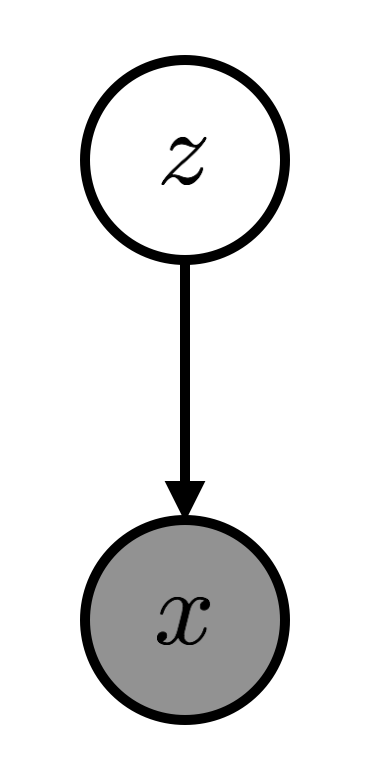
\includegraphics[width=0.15\textwidth]{images/predictive_coding/simple_latent_graphical_model.png}
    \caption{A graphical model denoting a latent variable model in which a single latent variable $z$ generates a single observed variable $x$. In predictive coding, we typically assume that $p(z)$ and $p(x|z)$ are Gaussian densities, and the generative mapping from $z$ to $x$ is a non-linear function.}
    \label{fig: simple_latent_model}
\end{figure}

\begin{equation}
	p (x | z) = \mathcal{N} (x; g(z), \sigma^2_x).
\end{equation}

\noindent Recall that in one dimension, a normal distribution takes the form

\begin{equation}
	\mathcal{N} (x; \mu, \sigma^2) = \frac{1}{\sqrt{2 \pi \sigma^2}} e^{-\frac{(x - \mu)^2}{2 \sigma^2}}.
	\label{eq: 1d gaussian}
\end{equation}

\noindent We will place a prior on $z$, which we also assume is a normal distribution with constant mean $\mu_p$ and constant variance $\sigma^2_p$:

\begin{equation}
	p (z) = \mathcal{N} (z; \mu_p, \sigma^2_p).
\end{equation}

\noindent To infer the posterior distribution of $z$, we can use Bayes' rule to invert the generative model:

\begin{equation}
	p (z | x) = \frac{p(x | z) p(z)}{p(x)},
\end{equation}

\noindent where the marginal distribution in the denominator is given as

\begin{equation}
	p (x) = \int p(x | z) p(z) dz.
	\label{eq: intractable integration}
\end{equation}

In general, computing the exact posterior distribution is computationally intractable due to the integration over $z$ in eq. \ref{eq: intractable integration}. Instead, we'll resort to variational inference\footnote{We are not actually using variational inference here, since the maximum of $p(z | x)$ must also be the maximum of $p(x, z)$ through the definition of conditional probability: $p(z|x) = \frac{p(x, z)}{p(x)}$, since $p(x)$ does not depend on the value of $z$. } to find the maximum (mode) of the posterior, otherwise known as the maximum a posteriori or MAP estimate. This is the \textit{most likely} estimate of the value of $z$. We will define our approximate distribution, a point mass estimate at $\mu_q$, as $q(z|x) = \delta (z = \mu_q)$, with the MAP estimate denoted as $\hat{\mu}_q$.

We want to maximize the evidence lower bound (ELBO), $\mathcal{L}$:

\begin{equation}
	\mathcal{L} = \mathbb{E}_{z \sim q(z|x)} \left[ \log p(x, z) - \log q(z|x) \right] = \mathbb{E}_{z \sim q(z|x)} \left[ \log p(x|z) + \log p(z) - \log q(z|x) \right] 
	\label{eq: elbo 1}
\end{equation}

\begin{equation}
	\mathcal{L} = \log \left( \frac{1}{\sqrt{2 \pi \sigma_x^2}} e^{-\frac{(x - g(\mu_q))^2}{2 \sigma_x^2}} \right) + \log \left( \frac{1}{\sqrt{2 \pi \sigma_p^2}} e^{-\frac{(\mu_q - \mu_p)^2}{2 \sigma_p^2}} \right)
	\label{eq: elbo 2}
\end{equation}

\begin{equation}
	\mathcal{L} = -\frac{1}{2} \log ( 2 \pi \sigma_x^2 )  - \frac{(x - g(\mu_q))^2}{2 \sigma_x^2} - \frac{1}{2} \log ( 2 \pi \sigma_p^2 ) -\frac{(\mu_q - \mu_p)^2}{2 \sigma_p^2}
	\label{eq: elbo 3}
\end{equation}

\begin{equation}
	\mathcal{L} = \frac{1}{2} \left( - \log ( \sigma_x^2 )  - \frac{(x - g(\mu_q))^2}{\sigma_x^2} - \log ( \sigma_p^2 ) -\frac{(\mu_q - \mu_p)^2}{\sigma_p^2} \right) + \text{const.}
	\label{eq: elbo 4}
\end{equation}

\noindent In going from eq. \ref{eq: elbo 1} to eq. \ref{eq: elbo 2}, we used the fact that $q(z|x)$ is a delta function, so the expectation becomes an evaluation at a single point, $z=\mu_q$. The expectation of $q(z|x)$ at this point is $1$, so $\log q(z|x)$ evaluates to $0$. To find the MAP estimate, we must solve the following optimization problem:

\begin{equation}
	\hat{\mu}_q = \text{argmax}_{\mu_q} \mathcal{L} =  \text{argmax}_{\mu_q} \frac{1}{2} \left( - \log ( \sigma_x^2 )  - \frac{(x - g(\mu_q))^2}{\sigma_x^2} - \log ( \sigma_p^2 ) -\frac{(\mu_q - \mu_p)^2}{\sigma_p^2} \right).
\end{equation}

\noindent To use first-order optimization methods, we must find the partial derivative of $\mathcal{L}$ w.r.t. $\mu_q$:

\begin{equation}
	\frac{\partial \mathcal{L}}{\partial \mu_q} = \frac{x - g(\mu_q)}{\sigma_x^2} \frac{d g}{d \mu_q} + \frac{\mu_q - \mu_p}{\sigma_p^2}
	\label{eq: 1d gradient}
\end{equation}

\noindent We see that we have two terms: \textbf{the first term moves the estimate toward agreement with the observation}, and \textbf{the second term moves the estimate toward agreement with the prior}. Each of these terms are weighted by their corresponding variances. In other words, inference (i.e. finding the optimal estimate of $\mu_q$) involves a weighted combination of \textit{bottom-up} and \textit{top-down} information. By repeatedly moving our estimate $\mu_q$ along this gradient, we can hopefully arrive at the MAP estimate $\hat{\mu}_q$. Note that we may not find the true value $\hat{\mu}_q$ if the optimization surface is non-convex. 

We would like to extend this single dimensional model to handle latent and observed variables of arbitrary size. In this setting, $\mathbf{x}$ and $\mathbf{z}$ are now vectors. The conditional likelihood, $p(\mathbf{x} | \mathbf{z}) = \mathcal{N} (\mathbf{x}; \bm{\mu}_\mathbf{x} = g(\mathbf{z}), \bm{\Sigma}_\mathbf{x})$ is now a multi-variate Gaussian distribution. The general form for this distribution is

 \begin{equation}
	\mathcal{N} (\mathbf{x}; \bm{\mu}, \bm{\Sigma}) = \frac{1}{(2 \pi)^{n/2} | \bm{\Sigma}|^{1/2}}  e^{-\frac{1}{2}(\mathbf{x} - \bm{\mu})^\intercal \bm{\Sigma}^{-1}(\mathbf{x} - \bm{\mu})},
	\label{eq: multi-variate gaussian}
\end{equation}

\noindent where $\bm{\Sigma}$ is the covariance matrix, $| \bm{\Sigma}|$ is the determinant of $\bm{\Sigma}$, and $n$ is the dimensionality of the vector $\mathbf{x}$. The prior on $\mathbf{z}$ is also a multi-variate Gaussian: $p(\mathbf{z}) = \mathcal{N} (\mathbf{z}; \bm{\mu}_p, \bm{\Sigma}_p)$. The MAP estimate is now a vector, $\hat{\bm{\mu}}_q$, of the most likely estimate of $\bm{\mu}_q$. To find this estimate, we must again optimize $\mathcal{L}$ w.r.t. $\bm{\mu}_q$. Repeating the steps above, the gradient, $\nabla_{\bm{\mu}_q} \mathcal{L}$, is given as:

\begin{equation}
	\nabla_{\bm{\mu}_q} \mathcal{L} =  \left( \frac{d g}{d \bm{\mu}_q} \right)^\intercal \bm{\Sigma}^{-1}_\mathbf{x} (\mathbf{x} - g(\bm{\mu}_q)) + \bm{\Sigma}^{-1}_p (\bm{\mu}_q - \bm{\mu}_p).
	\label{eq: multi-dimensional gradient}
\end{equation}

\section{The Dynamic Setting}

\section{Attention}

\section{Active Inference}

\section{Neural Implementation}

\subsection{Correspondence with Cortical Mircrocircuits}

\noindent \cite{bastos2012canonical} outlines ideas about correspondence between predictive coding and cortical microcircuits.
\newline

\noindent \cite{kanai2015cerebral} proposes that the pulvinar region of the thalamus is involved in setting precisions of predictions.
\newline

\noindent \cite{bogacz2017tutorial} gives an introductory tutorial to predictive coding with ideas about implementing predictive coding in neocortex.
\newline

\noindent \cite{whittington2017approximation} draws comparisons between backprop and predictive coding.
\newline

